\chapter{Monte Carlo-Informed Modelling for \isotope[90]{Y} Bremsstrahlung SPECT}
\label{chapterlabel3}

Chapter~\ref{chap:intro_material} described the principal limitations of \isotope[90]{Y} Bremsstrahlung \gls{spect}: the continuous photon spectrum makes conventional energy-window scatter correction unsuitable, high-energy photons undergo septal penetration and collimator scatter, and external Bremsstrahlung photons may be emitted away from the original decay site as the $\beta^-$ particle traverses tissue. This chapter develops the practical \glsentryshort{spect} model used later for joint \glsentryshort{pet}/\glsentryshort{spect} reconstruction. It addresses two specific components: a \glsentryshort{simind}-derived estimate of non-primary counts and an image-space approximation to Bremsstrahlung range blur.

The resulting model is
\begin{equation} \label{eq:brems_forward_model}
    \bar y(x) = A_{\mathrm{prim}}K_{\mathrm{brem}}x+b_{\mathrm{MC}}
\end{equation}
where $A_{\mathrm{prim}}$ contains attenuation, geometric projection, the intrinsic detector response and the geometric collimator response; $K_{\mathrm{brem}}$ is the image-space range-blur operator and $b_{\mathrm{MC}}$ represents detected counts not described by this primary-event model. The latter includes patient scatter, collimator scatter and septal penetration, so these effects are not also included in $A_{\mathrm{prim}}$. It is therefore referred to throughout as a non-primary additive term, rather than as patient scatter alone.

The two components in Equation~\ref{eq:brems_forward_model} are estimated in a preparatory stage. Once estimated, both the acquisition model and $b_{\mathrm{MC}}$ are fixed during the target reconstruction. The purpose of the reconstruct--simulate loop below is to prepare an object- and acquisition-specific additive estimate, which avoids altering the objective function, and therefore the solution, during reconstruction.


\section{Pre-Reconstruction Estimation of Non-Primary Counts}
\label{sec:additive_corrections}

Monte Carlo estimates of scatter and penetration can be combined with a faster analytic projector by alternating reconstruction and simulation \cite{dewarajaImprovedQuantitative90Y2017}. The approach used here follows that established principle. The practical questions addressed in this chapter are how to initialise the simulation for a different acquisition protocol and how to prevent an alternating update from becoming unstable before the final additive term is frozen.

\subsection{Learned initialisation}

The scatter-derived initial estimate $b^{(0)}$ is produced by the convolutional neural network of Xiang et al., which predicts scatter projections from measured emission data and \glsentryshort{ct}-derived attenuation information \cite{xiangDeepNeuralNetwork2020}. The available network was trained for a different scanner, collimator and energy-window configuration from the acquisitions used in this thesis. Its output is consequently treated only as a computationally inexpensive warm start for the broader non-primary term, not as a final quantitative correction or as an independently validated contribution. The adapted \glsentryshort{sirf} inference workflow is documented in Appendix~\ref{app:scatter_dl}.

\subsection{Reconstruct--simulate refinement}
\label{subsec:additive_refinement}

Starting from $b^{(0)}$, an outer iteration consists of the following operations:
\begin{enumerate}
    \item reconstruct an activity estimate $x^{(k)}$ using the current additive term $b^{(k)}$;
    \item smooth the intermediate image with an isotropic $5\,\mathrm{mm}$-\gls{fwhm} Gaussian and restrict it to the body mask, giving $\widetilde x^{(k)}$;
    \item use the smoothed image as the source distribution for a  \glsentryshort{simind} simulation; and
    \item extract a newly simulated non-primary estimate $\widehat b^{(k+1)}$ and update the running estimate.
\end{enumerate}
Each intermediate reconstruction used 12 staggered subsets and 10 epochs (120 subset updates), warm-started from the preceding outer iterate. Ten outer iterations were used as a pre-specified computational budget. This endpoint is not presented as evidence of asymptotic convergence. The simulations were driven from Python using the interface described in Appendix~\ref{app:simind_python_connector}.

At outer iteration $k$, one simulation produces the total simulated detected projection counts $p_{\mathrm{tot}}^{(k)}$ and the attenuated, geometrically collimated primary component $p_{\mathrm{geo}}^{(k)}$. Inspired by the work by Dewaraja et. al in \cite{dewarajaImprovedQuantitative90Y2017}, the Monte Carlo projections are first placed on the scale of the analytic acquisition model $A_{\star}=A_{\mathrm{prim}}K_{\mathrm{brem}}$. Let $\mathcal I_k$ contain bins with non-zero $p_{\mathrm{geo},i}^{(k)}$ after the lowest and highest 5\% of the per-bin ratios $(A_{\star}\widetilde x^{(k)})_i/ p_{\mathrm{geo},i}^{(k)}$ have been excluded. The scalar calibration is
\begin{equation}
    s^{(k)} =
    \frac{\sum_{i\in\mathcal I_k}(A_{\star}\widetilde x^{(k)})_i}
         {\sum_{i\in\mathcal I_k}p_{\mathrm{geo},i}^{(k)}},
    \label{eq:simind_scale}
\end{equation}
and the newly simulated additive term is
\begin{equation}
    \widehat b^{(k+1)} =
    s^{(k)}\!\left(p_{\mathrm{tot}}^{(k)}-p_{\mathrm{geo}}^{(k)}\right).
    \label{eq:simind_additive}
\end{equation}
Thus, Equation~\ref{eq:simind_additive} includes all simulated counts outside the geometrically collimated primary component; it is not an estimate of patient Compton scatter alone. Before simulation, the body mask was formed by thresholding the attenuation map at $0.05\,\mathrm{cm}^{-1}$, applying a morphological opening of radius two voxels and retaining the largest connected component in order to remove \gls{ct} acquisition noise and the patient bed.

\subsection{Under-relaxed updates}
\label{subsec:additive_damping}

The most direct update replaces the running estimate with the new simulation,
\begin{equation}
    b^{(k+1)}=\widehat b^{(k+1)}.
    \label{eq:additive_full_update}
\end{equation}
Using this methods, we observed some divergence in non-primary additive term where subsequent updates would result in increasing oscillating underestimation followed by overestimation. To reduce the resulting iteration-to-iteration variation, an under-relaxed update was used,
\begin{equation}
    b^{(k+1)}=(1-\alpha)b^{(k)}+\alpha\widehat b^{(k+1)},
    \qquad \alpha=0.2.
    \label{eq:additive_damped_update}
\end{equation}
The value $\alpha=0.2$ was selected heuristically rather than through an optimisation study.

Figure~\ref{fig:nema_scatter_est} shows the diagnostic that motivated this choice. With full replacement, the scale of successive projection profiles oscillates and grows rapidly. By the fourth outer iteration, the estimated additive profile well exceeds the measured total-emission profile. Under-relaxation keeps the profiles bounded over the ten-step refinement budget and suppresses the large iteration-to-iteration swings.

\begin{figure}[H]
    \centering
    \begin{subfigure}[b]{0.92\textwidth}
        \centering
        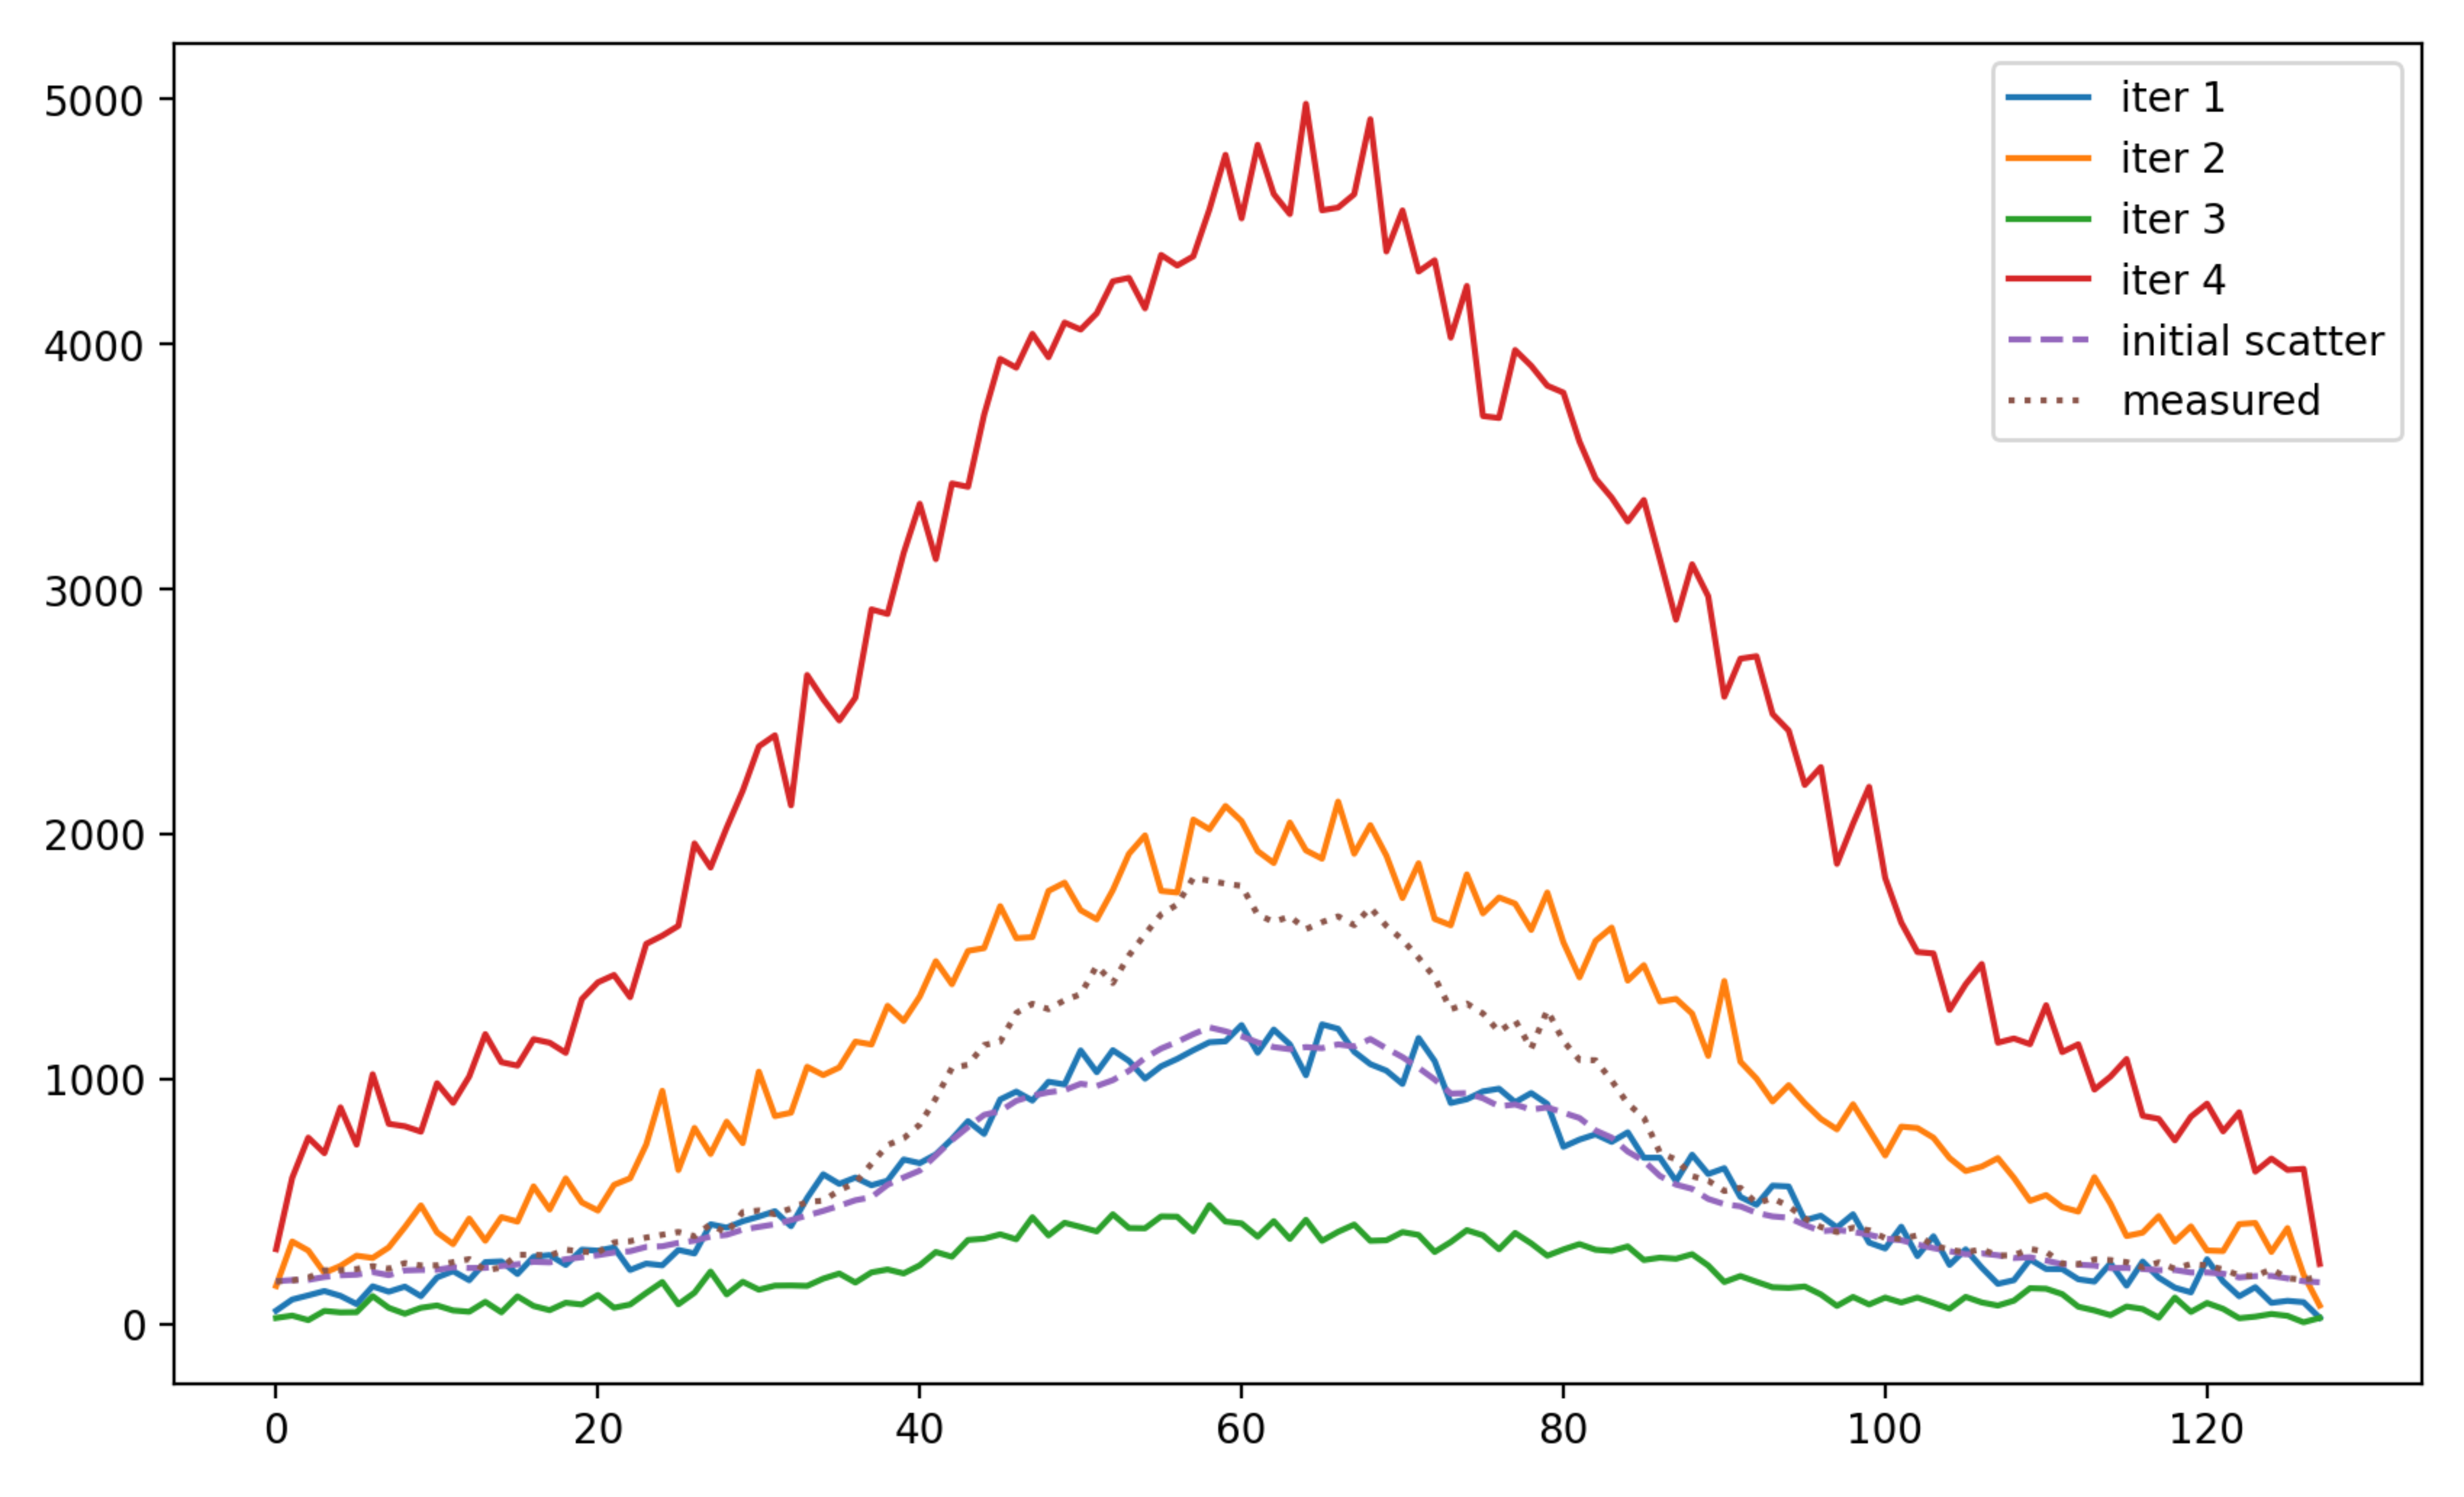
\includegraphics[width=\linewidth]{figures/Chapter3/offline_scatter_replace.png}
        \caption{Full replacement, $\alpha=1$.}
    \end{subfigure}

    \begin{subfigure}[b]{0.92\textwidth}
        \centering
        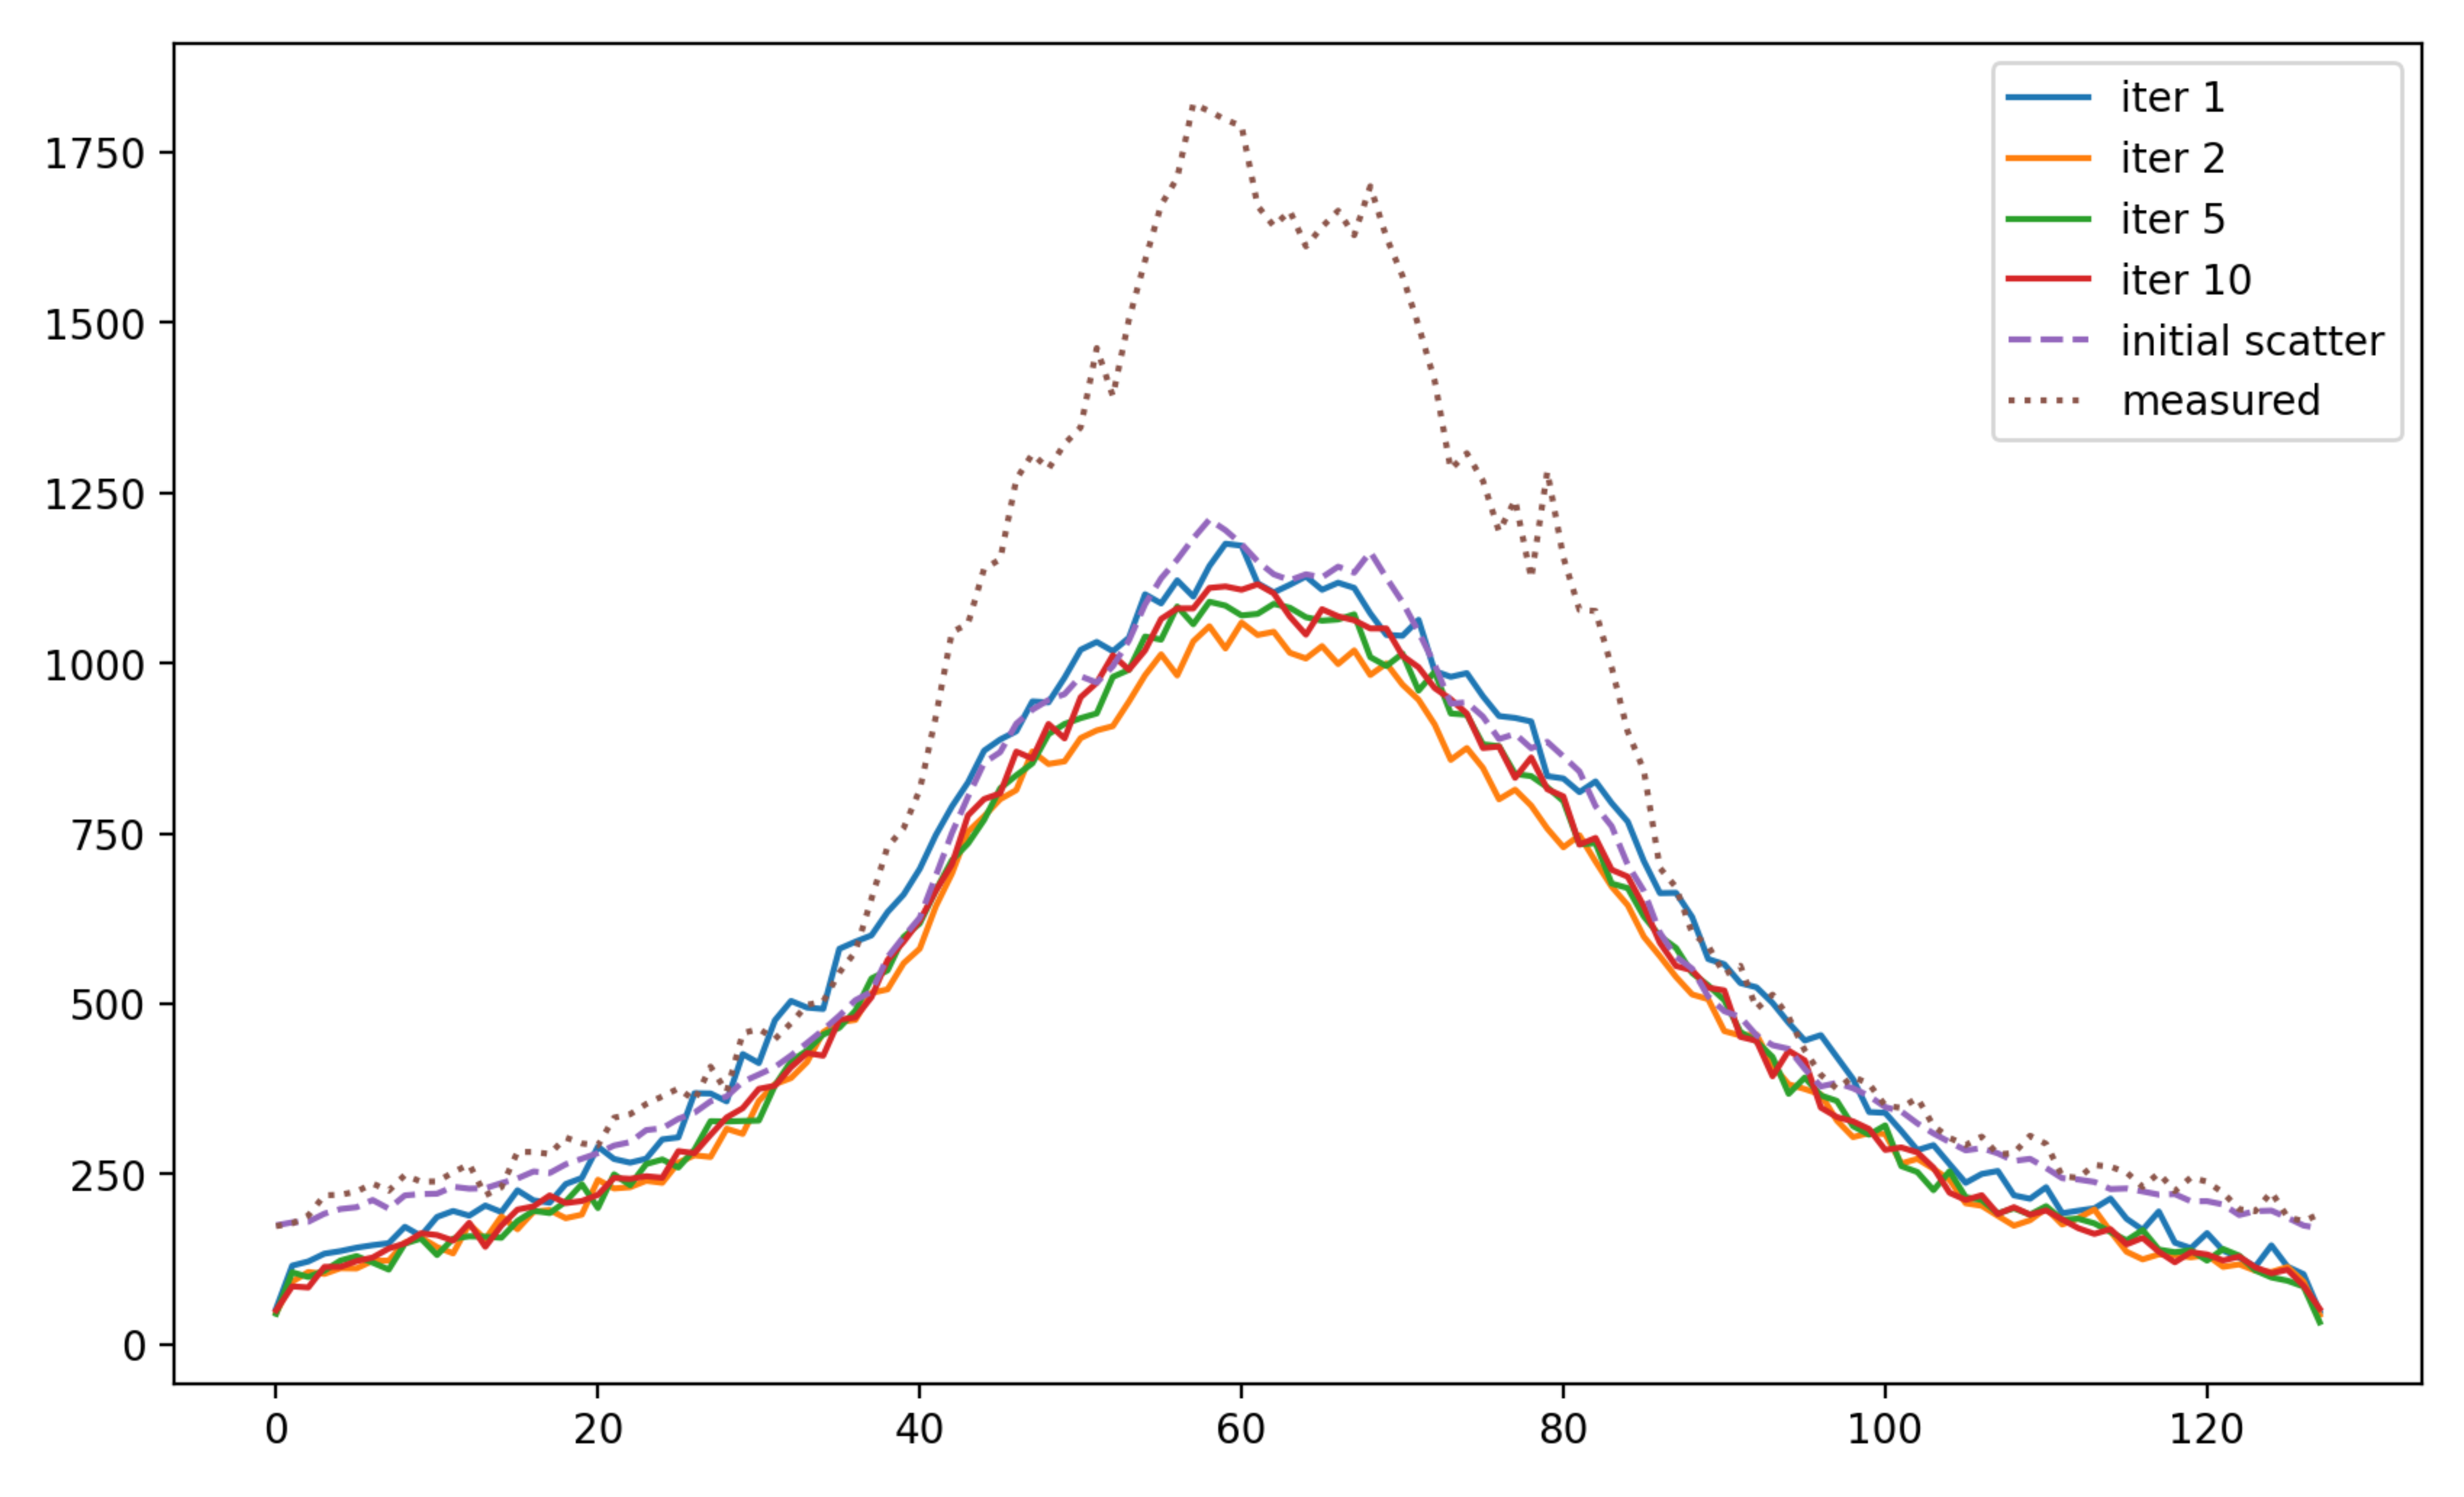
\includegraphics[width=\linewidth]{figures/Chapter3/offline_scatter_damped.png}
        \caption{Under-relaxed update, $\alpha=0.2$.}
    \end{subfigure}
    \caption{Projection-domain behaviour of the preparatory additive-term refinement for a measured NEMA phantom. Coloured curves are profiles of the estimated non-primary term $b^{(k)}$; every displayed iteration is one outer step of the preparatory reconstruct--simulate loop. Profiles are summed over views at an axial position through the spheres; the horizontal coordinate is the tangential detector bin and the vertical coordinate is counts. Full replacement
    produces large alternating changes within four outer iterations, whereas the under-relaxed profiles remain bounded through the tenth outer iteration.}
    \label{fig:nema_scatter_est}
\end{figure}

After the tenth outer iteration, the final estimate is denoted $b_{\mathrm{MC}}=b^{(10)}$ and is frozen. No additional SIMIND simulation or additive-term update is performed during the target reconstruction. This makes $b_{\mathrm{MC}}$ a data- and activity-dependent plug-in estimate and the target reconstruction has a fixed objective.


\section{Image-Space Bremsstrahlung Range Blur}
\label{sec:brem_range_blur}

External Bremsstrahlung photons may be emitted after the $\beta^-$ particle has travelled away from the \isotope[90]{Y} decay site, whereas internal Bremsstrahlung is emitted at the decay site. The displacement distribution of the external component is energy dependent, as illustrated in Figure~\ref{fig:source_to_emission}, and its net contribution adds a resolution loss distinct from the collimator--detector response \cite{raultFastSimulationYttrium902010,rongDevelopmentEvaluationImproved2012, dewarajaImpactInternalBremsstrahlung2018}. Detailed Monte Carlo projectors can model this transport directly, but repeatedly evaluating such a model is impractical for the iterative and joint reconstructions developed later in this thesis.

\begin{figure}[H]
    \centering
    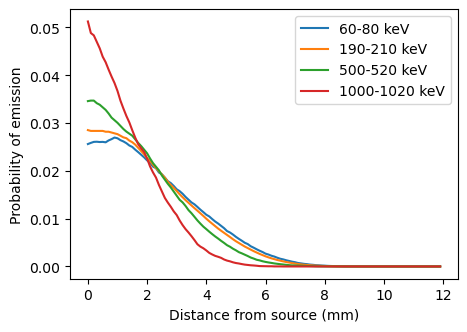
\includegraphics[width=0.68\linewidth]{figures/Chapter3/source_to_emission.png}
    \caption{Probability of external Bremsstrahlung photon emission as a function
    of displacement from the \isotope[90]{Y} decay site for four photon-energy
    intervals. Curves were derived from the fast-simulation data reported by
    Rault et al.\ \cite{raultFastSimulationYttrium902010}.}
    \label{fig:source_to_emission}
\end{figure}

\subsection{Primary collimator--detector response}

The analytic primary projector blurs each source plane with a depth-dependent Gaussian point-spread function that represents the intrinsic and geometric components of the \gls{cdr}; scatter and penetration remain in $b_{\mathrm{MC}}$. For photon energy $E$ and source--collimator distance $h$, this \gls{psf} is
\begin{equation}
    K_{\mathrm{cdr}}(\mathbf r;h,E)=
    \mathcal N\!\left(\mathbf r;\mathbf 0,
    \sigma_{\mathrm{cdr}}(h;E)^2\mathbb I\right),
    \label{eq:cdr_psf}
\end{equation}
an isotropic Gaussian in the detector plane whose standard deviation $\sigma_{\mathrm{cdr}}$ sets the blur width. \gls{stir} models this width as affine in depth,
\begin{equation}
    \sigma_{\mathrm{cdr}}(h;E)=c_0(E)+c_1(E)h,
    \label{eq:cdr_linear}
\end{equation}
so the two coefficients $c_0(E),c_1(E)$ fully specify the depth-dependent \gls{cdr} for a given energy. Physically, however, the \gls{cdr} standard deviation is the quadrature sum of a depth-independent intrinsic term and a depth-dependent parallel-hole geometric term, $\sqrt{\sigma_{\mathrm{int}}(E)^2+\sigma_{\mathrm{geo}}(h;E)^2}$, which is not affine in $h$. We therefore fit \gls{stir}'s affine model \eqref{eq:cdr_linear} by least squares over $h\in[2,20]\,\mathrm{cm}$ to this quadrature sum, evaluated from the measured intrinsic and analytic geometric standard deviations. Over this range the quadrature sum is close to linear, so the affine surrogate reproduces the conventional distance dependence of the collimator response to within the accuracy required inside the projector \cite{angerSensitivityResolutionLinearity1966}.

\subsection{Effective Gaussian range-kernel approximation}
\label{subsec:brem_specific_blur}

An exact reduced transport model would distinguish internal Bremsstrahlung, represented by an identity component at the decay site, from the displaced external component. The reconstruction implementation instead uses one zero-mean isotropic Gaussian as an empirical surrogate for their net central-response broadening,
\begin{equation}
    G_{\mathrm{brem}}(\mathbf r)=
    \mathcal N\!\left(\mathbf r;\mathbf 0,
    \sigma_{\mathrm{eff}}^2\mathbb I\right).
    \label{eq:brem}
\end{equation}
The Gaussian form is motivated by the external-photon displacement distributions of Rault et al., while its effective width was estimated from the water-equivalent Monte Carlo response study described below \cite{raultFastSimulationYttrium902010}. 

The resulting operator $K_{\mathrm{brem}}$ is a three-dimensional Gaussian convolution applied in image space. It is composed with the analytic projector in the forward operation and with the analytic backprojector in reverse order in the adjoint,
\begin{equation}
    A_{\star}=A_{\mathrm{prim}}K_{\mathrm{brem}},
    \qquad
    A_{\star}^{\mathsf T}=K_{\mathrm{brem}}^{\mathsf T}
    A_{\mathrm{prim}}^{\mathsf T}.
    \label{eq:brem_matched_operator}
\end{equation}
For the symmetric Gaussian kernel, $K_{\mathrm{brem}}^{\mathsf T}=K_{\mathrm{brem}}$. This construction therefore preserves a matched forward--adjoint pair while adding only an image-space convolution to each operation.

\subsection{Projection-response calibration and cross-code comparison}
\label{subsec:brem_blur_validation}

The approximation was assessed using spherical \SI{2.2}{\milli\metre} \isotope[90]{Y} source distributions in water, inspired by the physical phantoms produced by Rong et al in \cite{rongDevelopmentEvaluationImproved2012} \footnote{\SI{2.2}{\milli\metre} is chosen here because it is double the approximate maximum bremsstrahlung range of \isotope[90]{Y} electrons in water. Using a point source, as is usual in such experiments, would result in no photons becasuse of a lack of scattering material.}, and four source--collimator distances ($2$, $5$, $10$ and $20\,\mathrm{cm}$). Detector-plane response widths were compared for three energy windows representing standard practice at The Christie NHS Foundation Trust, Oxford University Hospitals Foundation Trust and The Royal Surrey NHS Foundation Trust. These were $[39.8,126.6]$, $[50,150]$ and $[75,225]\,\mathrm{keV}$, respectively. The four models were GATE Monte Carlo, SIMIND Monte Carlo, \glsentryshort{stir} with the geometric \glsentryshort{cdr} alone, and \glsentryshort{stir} with the geometric response composed with $K_{\mathrm{brem}}$. GATE provides the response used to calibrate and check the effective width, while SIMIND provides a cross-code comparison.

Figure~\ref{fig:gaussian_bremss_range} reports the fitted detector-plane standard deviation. The geometric-only STIR model is systematically narrower than both Monte Carlo responses. Adding the image-space kernel moves the STIR prediction towards the GATE and SIMIND values at every evaluated distance and for all three energy windows. The agreement is not exact, particularly for the widest window at large distance, but the comparison supports the Gaussian kernel as a practical reduced-order representation of the missing net response broadening. 

\begin{figure}[H]
    \centering
    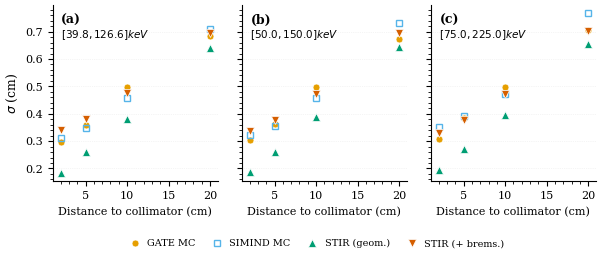
\includegraphics[width=\linewidth]{figures/Chapter3/Gaussian_bremss_range.png}
    \caption{Projection space Gaussian \gls{psf} standard deviation, $\sigma$ (cm), against
    source--collimator distance for (a) $[39.8,126.6]$, (b) $[50,150]$ and
    (c) $[75,225]\,\mathrm{keV}$. Markers show GATE MC, SIMIND MC, STIR with the
    geometric response, and STIR with the geometric response plus the image-space
    effective kernel. The geometric-only STIR projector
    underestimates the width; composing it with the image-space
    Bremsstrahlung kernel substantially reduces the net width discrepancy across the
    evaluated distances and windows.}
    \label{fig:gaussian_bremss_range}
\end{figure}


\section{Scope, Limitations and Deployment}
\label{sec:brems_deployment}

The work in this chapter is only a component-level commissioning study. Iterative Monte Carlo estimation of scatter is established methodology, and under-relaxation is a standard numerical device. The contribution here is the integration of a learned initial estimate with a calibrated SIMIND refinement, and the empirical identification and suppression of unstable full replacement. Likewise, the physical existence of Bremsstrahlung range broadening is established. The contribution is an inexpensive fixed-width effective Gaussian surrogate that can be composed with a standard matched projector, calibrated against GATE and cross-checked against SIMIND.

Several limitations follow from these choices. The network output is used outside its training protocol and is only a scatter-derived initialisation. Because the update is damped, it could continue to influence the finite-budget estimate to some extent, however we posit that this would be minimal after simulate--reconstruct 10 iterations. The scalar calibration in Equation~\ref{eq:simind_scale} cannot correct spatially varying differences between SIMIND and the analytic projector which may exist. The relaxation factor and ten-iteration budget were fixed heuristically, and Figure~\ref{fig:nema_scatter_est} is a stability diagnostic rather than a convergence proof. The range kernel is isotropic and water-equivalent, so it does not model material-dependent transport in lung or bone, nor the detailed angular and spectral structure represented by a full Monte Carlo projector. Future work could include the addition of anisotropic bremsstrahlung simulation methods such as that by Lim et al. \cite{lim_y-90_2018}. Finally, the analysis isolates selected model components and does not by itself establish improved clinical quantification.

The configuration carried forward is as follows: a learned additive estimate is refined for ten outer iterations using SIMIND and Equation~\ref{eq:additive_damped_update}; the final non-primary term is frozen; and the effective range kernel is added to the SPECT acquisition model. Chapter~\ref{chapter:paper} uses this fixed model for the joint \isotope[90]{Y} \glsentryshort{pet}/\glsentryshort{spect} experiments.


\section{Summary}

This chapter established the two Bremsstrahlung-specific components required by the later reconstruction experiments. First, a learned projection estimate was used to initialise object- and acquisition-specific SIMIND simulations of non-primary contamination. Full replacement was unstable in the measured NEMA example, whereas an under-relaxed update with $\alpha=0.2$ remained bounded over the prescribed refinement budget. The resulting additive estimate was then frozen. Second, Monte Carlo response broadening was represented by a image-space Gaussian. Composing this kernel with the analytic projector brought projected response widths substantially closer to GATE and SIMIND across three energy windows. Together, these components define the fixed \isotope[90]{Y} Bremsstrahlung \glsentryshort{spect} model used in the final joint-reconstruction study.
